%%% %%%%%%%%%%%%%%%%%%%%%%%%%%%% %%%
%%% Main Chapter 2 : Challenges  %%%
%%% %%%%%%%%%%%%%%%%%%%%%%%%%%%% %%%
\chapter{Darstellung der Evolution historischer Betriebssysteme}
\label{chap:challenges}

Der Fokus dieser Arbeit liegt auf der praxisnahen Vermittlung der historischen Entwicklung der Betriebssysteme und nicht der Entwicklung selbst. Daher wird auf diese hier nicht gesondert eingegangen.

Dem interessierten Leser bietet jedoch der Artikel "`History of Microsoft Windows"' der englischsprachigen Wikipedia\footnote{\url{http://en.wikipedia.org/wiki/History_of_Microsoft_Windows}} einen guten Einstieg.
Detailliertere Informationen finden sich zudem in \cite{WinInt1} und auf \cite{WinHistory}.

%%%%%%%%%%%%%%%%%%%%%%%%%%%%%%%%%%%%%%%%%%%%%%%%%%%%%%%%%%%%%%%%%%%%%%%%%%%%%%%%%%%%%%%%%%%%%%%%%%%%%%%%%
\section{Aufgabenstellung}
\label{sec:aims}
%%%%%%%%%%%%%%%%%%%%%%%%%%%%%%%%%%%%%%%%%%%%%%%%%%%%%%%%%%%%%%%%%%%%%%%%%%%%%%%%%%%%%%%%%%%%%%%%%%%%%%%%


		Ziel ist es die historischen Betriebssysteme den Studenten möglichst originalgetreu zur Verfügung zu stellen. 
		Im Rahmen dieser Arbeit sollen daher insgesamt sechs verschiedene Betriebssysteme installiert werden. 
		Zu jedem sollen im Durchschnitt zwei verschiedene Experimente angeboten werden, anhand derer Studenten herausragende Merkmale studieren und vor allem erleben können.

		Der vorgesehene Anwendungsfall ist die Übernahme der in dieser Arbeit erzeugten VMs mitsamt Experimenten in das InstantLab\footnote{\url{http://experiments.instantlab.org/about}}. 
		In dieser Cloud-Umgebung für virtuelle Maschinen können ohne großen Aufwand die Experimente im Webbrowser durchgeführt werden. 
		Zudem soll durch die zentrale Verwaltung auf einer einheitlichen Hardwareplattform der Wartungsaufwand stark reduziert werden.
		Von Vorteil ist hier die Verwendung von OpenStack, da durch diesen einheitlichen Standard ein Vendor-Lock-in größtenteils vermieden wird und ohne größere Schwierigkeiten zwischen eigener und fremder Hardware auf einer Plattform-as-a-Service gewechselt werden kann.


%%%%%%%%%%%%%%%%%%%%%%%%%%%%%%%%%%%%%%%%%%%%%%%%%%%%%%%%%%%%%%%%%%%%%%%%%%%%%%%%%%%%%%%%%%%%%%%%%%%%%%%%%
\section{Anforderungen}
\label{sec:requirements}
%%%%%%%%%%%%%%%%%%%%%%%%%%%%%%%%%%%%%%%%%%%%%%%%%%%%%%%%%%%%%%%%%%%%%%%%%%%%%%%%%%%%%%%%%%%%%%%%%%%%%%%%%

		Aus den oben genannten Zielen ergeben sich detaillierte Anforderungen an die Beschaffenheit der in den virtuellen Maschinen verpackten Experimente sowie die Funktionalität des InstantLabs.

		Grundsätzlich werden wir üblich funktionale und nicht-funktionale Anforderungen unterschieden;
		spezifische didaktische Anforderungen werden nicht behandelt und fallen in den Aufgabenbereich des jeweiligen Kursleiters. 

		%%%%%%%%%%%%%%%%%%%%%%%%%%%%%%
		\subsection{Funktionale Anforderungen}
		%%%%%%%%%%%%%%%%%%%%%%%%%%%%%%


		Grundsätzlich können drei Akteure identifiziert werden:

		\begin{enumerate}
			\item \emph{Student} Teilenhmer einer Lehrveranstaltung. Von diesem werden Experimente durchgeführt und Ergebnisse zur Benotung eingereich.
			\item \emph{Administrator} Verantwortlich für den Betrieb des InstantLabs und Kontaktperson bei technischen Problemen. Außerdem zuständig für die Erteilung und den Entzug von Zugriffsrechten.
			\item \emph{Kursleiter} Legt Experimente für Studenten an, hierzu werden Templates virtueller Maschinen eingerichtet und Datenträgerimages installiert. Benotet Studenten nach Abgabe der Ergebnisse.
		\end{enumerate}


			\begin{figure}[h]
				\begin{center}
					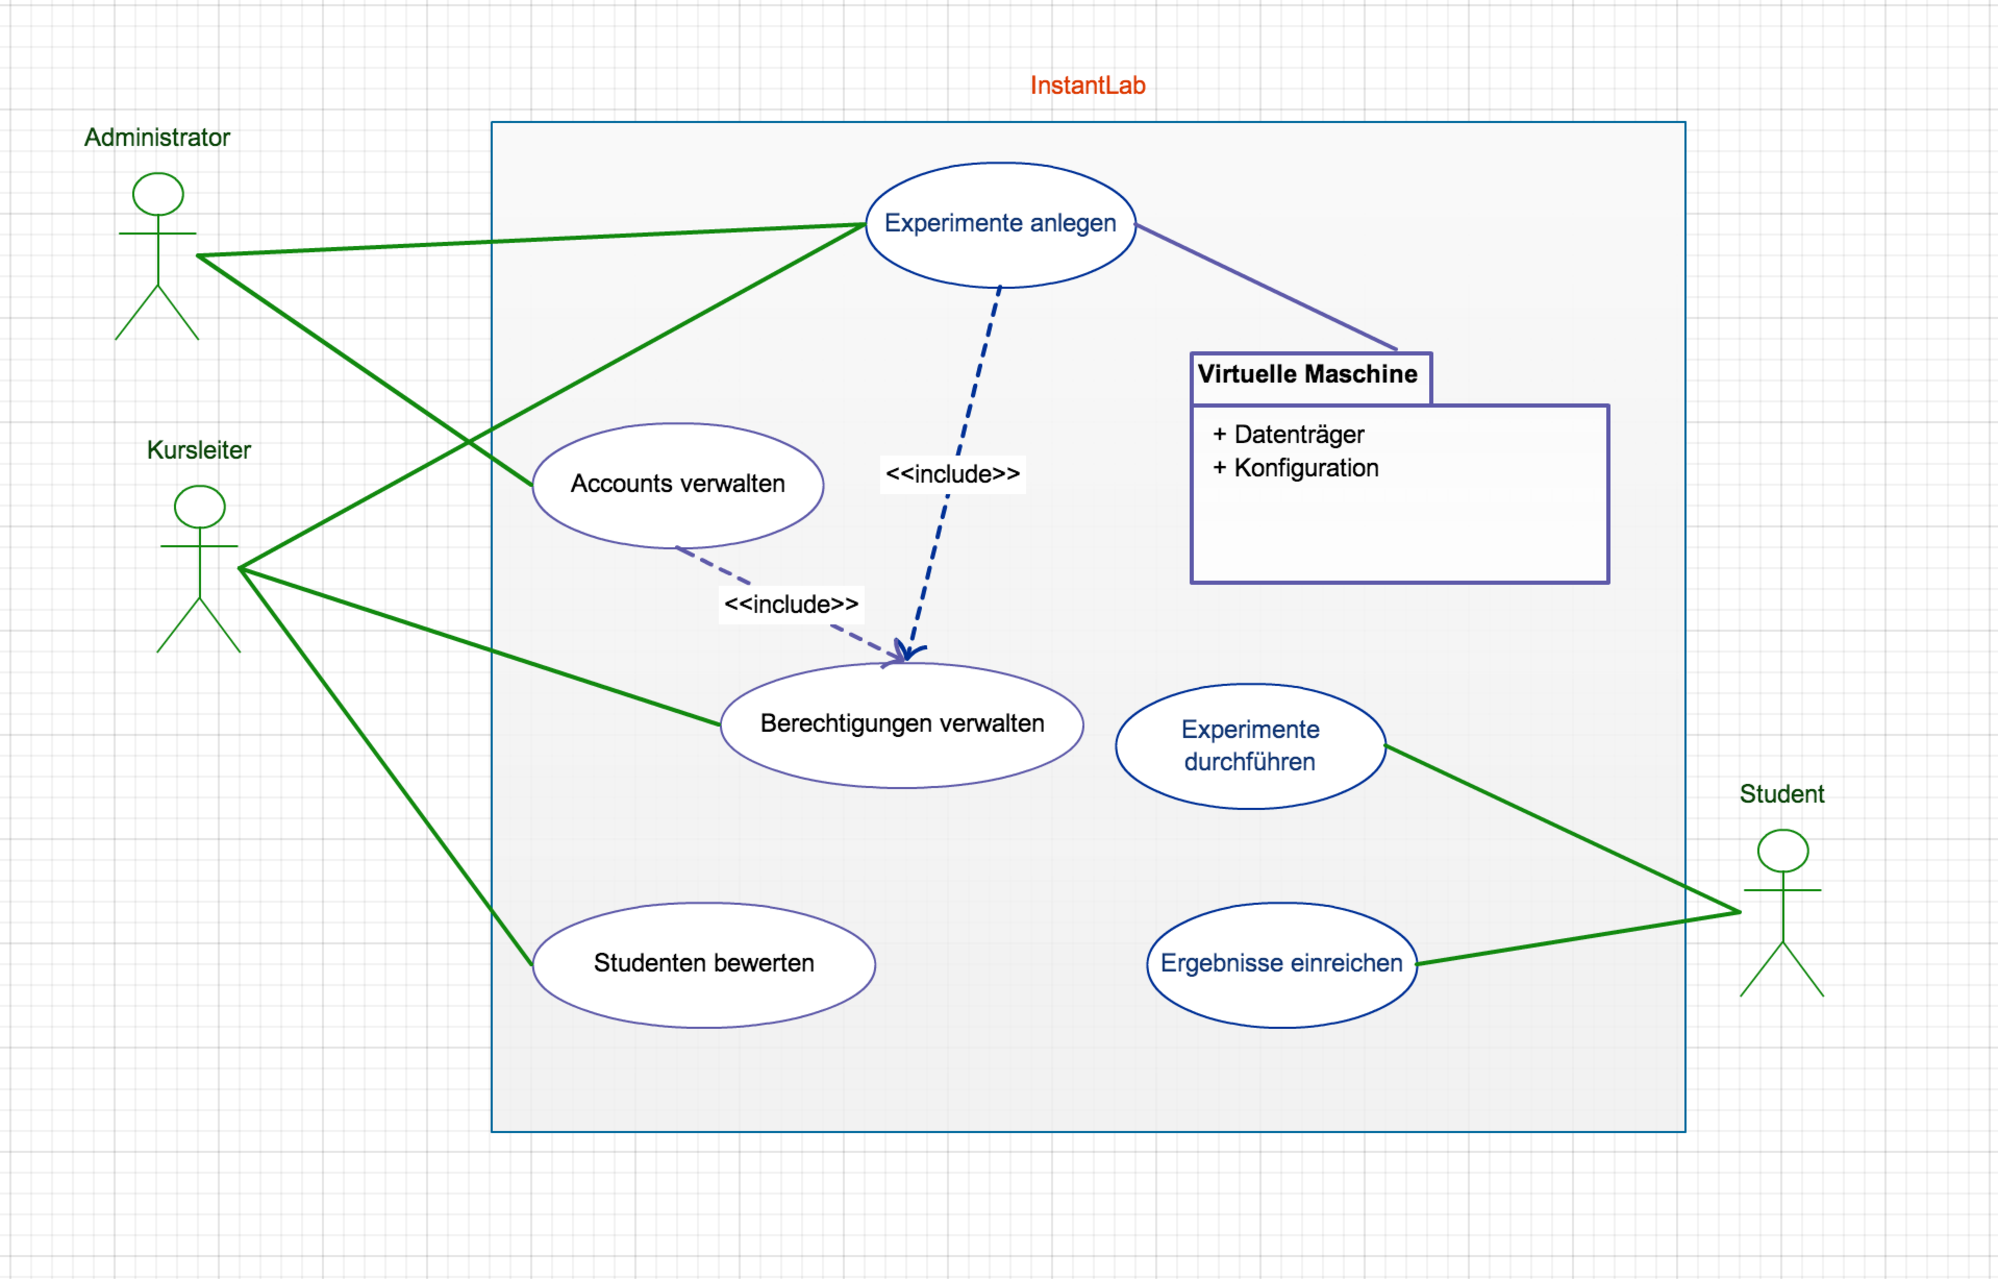
\includegraphics[width=\textwidth]{img/usecases}
					\caption{Use Case Diagramm des InstantLabs}
					\label{fig:instantlab-usecases}
				\end{center}
			\end{figure}


		%%%%%%%%%%%%%%%%%%%%%%%%%%%%%%
		\subsection{Nicht-Funktionale Anforderungen}
		%%%%%%%%%%%%%%%%%%%%%%%%%%%%%%

		\begin{enumerate}
			\item \emph{Isolation} Ein Experiment darf Andere nicht beeinflussen. Insbesondere dürfen Fehler bei der Durchführung keine Auswirkung auf die Durchführung des Experiments bei anderen Teilnehmern haben.
			\item \emph{Tamper-Proof} Auch bei böswilliger Manipulation muss die Isolation gewährleistet werden, auch muss eine faire Bewertung und Schutz vor Betrug gewährleistet werden. Zudem müssen Maßnahmen gegen DOS-Angriffe durch Erzeugung von Überlast in den VMs und somit auf dem Execution Hosts getroffen werden. 
			\item \emph{Geschwindigkeit} Der Zugriff erfolgt über das Internet. Eine unangenehme User Experience durch lange Ladezeiten, schlechte Responsiveness oder Darstellungsfehler stört die Konzentration und verschlechtert das Lernergebnis. Daher muss insbesondere auf eine schnelle Anbindung und geringe Übertragungsrate des VNC-Protokolls geachtet werden.
		\end{enumerate}
	

%%%%%%%%%%%%%%%%%%%%%%%%%%%%%%%%%%%%%%%%%%%%%%%%%%%%%%%%%%%%%%%%%%%%%%%%%%%%%%%%%%%%%%%%%%%%%%%%%%%%%%%%%
\section{Vergleichbare Systeme}
\label{sec:solutions}
%%%%%%%%%%%%%%%%%%%%%%%%%%%%%%%%%%%%%%%%%%%%%%%%%%%%%%%%%%%%%%%%%%%%%%%%%%%%%%%%%%%%%%%%%%%%%%%%%%%%%%%%%
		


	Zum Vergleich werden die zwei wichtigsten Anbieter von Massive Online Open Courses aufgeführt. 
	Während das Ziel des InstantLabs die Begleitung einer bestehenden Lehrveranstaltung ist, werden dort komplette Kurse für die Allgemeinheit angeboten. 
	Im Gegensatz zu den Lehrveranstaltungen an Universitäten, für die eine Immatrikulation notwendig ist, existieren keine Kenntnisse über den User, seine Vorkenntnisse und bisherigen Noten. 

	Auch bietet keines der Systeme bislang Live-Experimente an, meist werden lediglich Übungsaufgaben gestellt, die zum Beispiel mit Stift und Papier bearbeitet werden müssen. 

	Eine besondere Neugikeit von InstantLab besteht daher in der Möglichkeit, jederzeit nach einem Login neue Instanzen eines Experiments per Mausklick zu erzeugen. 
	Eine bestimmte Hardwarekonfiguration oder manuelle Installation von Software entfällt im Gegensatz zum bisherigen Übungsbetrieb.
		
	Bemühungen die Geschichte von Computern und insbesondere die Entwicklung von Software zu Archivieren und zu Konservieren werden ebenfalls vom Computer History Museum in Mountain View unternommen.
	Unlängst hat dieses den Source Code von MS DOS sowie Microsoft Word der ersten Generation veröffentlicht\footnote{\url{http://www.computerhistory.org/press/ms-source-code.html}}.

		\subsection{Udacity}

			Bei Udacity handelt es sich um ein vom Stanford-Professor Sebastian Thrun geschaffene Plattform zur Wissensvermittlung über das Internet.
			Diese ist an den universitären Lehrbetrieb angelehnt, so gibt es Videoaufnahmen von Vorlesungen, Begleitlektüren und ein Diskussionsforum für alle Teilnehmer. 


			Zudem wird ein Übungssystem angeboten, bei dem den Teilnehmern der Veranstaltung regelmäßig Aufgaben gestellt werden. Diese müssen selbstständig bearbeitet und anschließend über das System abgegeben werden.
			Über dieses System erfolgt nach einer Korrektur, die in den meisten Fällen automatisch erfolgt, eine Bewertung.
			Hierdurch kann der Lernfortschritt effizient kontrolliert werden. %Aufgabenabgabesystem

			Die erste dort angebotene Lehrveranstaltung war die Vorlesung "`CS101 - Intro to Computer Science: Building a Search Engine"' der Stanford University im Jahr 2011\footnote{http://de.wikipedia.org/wiki/Udacity}.

			Nach wie vor liegt der Fokus des Angebots in erster Linie auf dem Bereich Informatik, mittlerweile werden aber auch Kurse in anderen Fachbereichen, z.B. "`Intro to the Design of Everyday Things"' von Don Norman oder "`How to Build a Startup"' angeboten.


			\begin{figure}[h]
				\begin{center}
					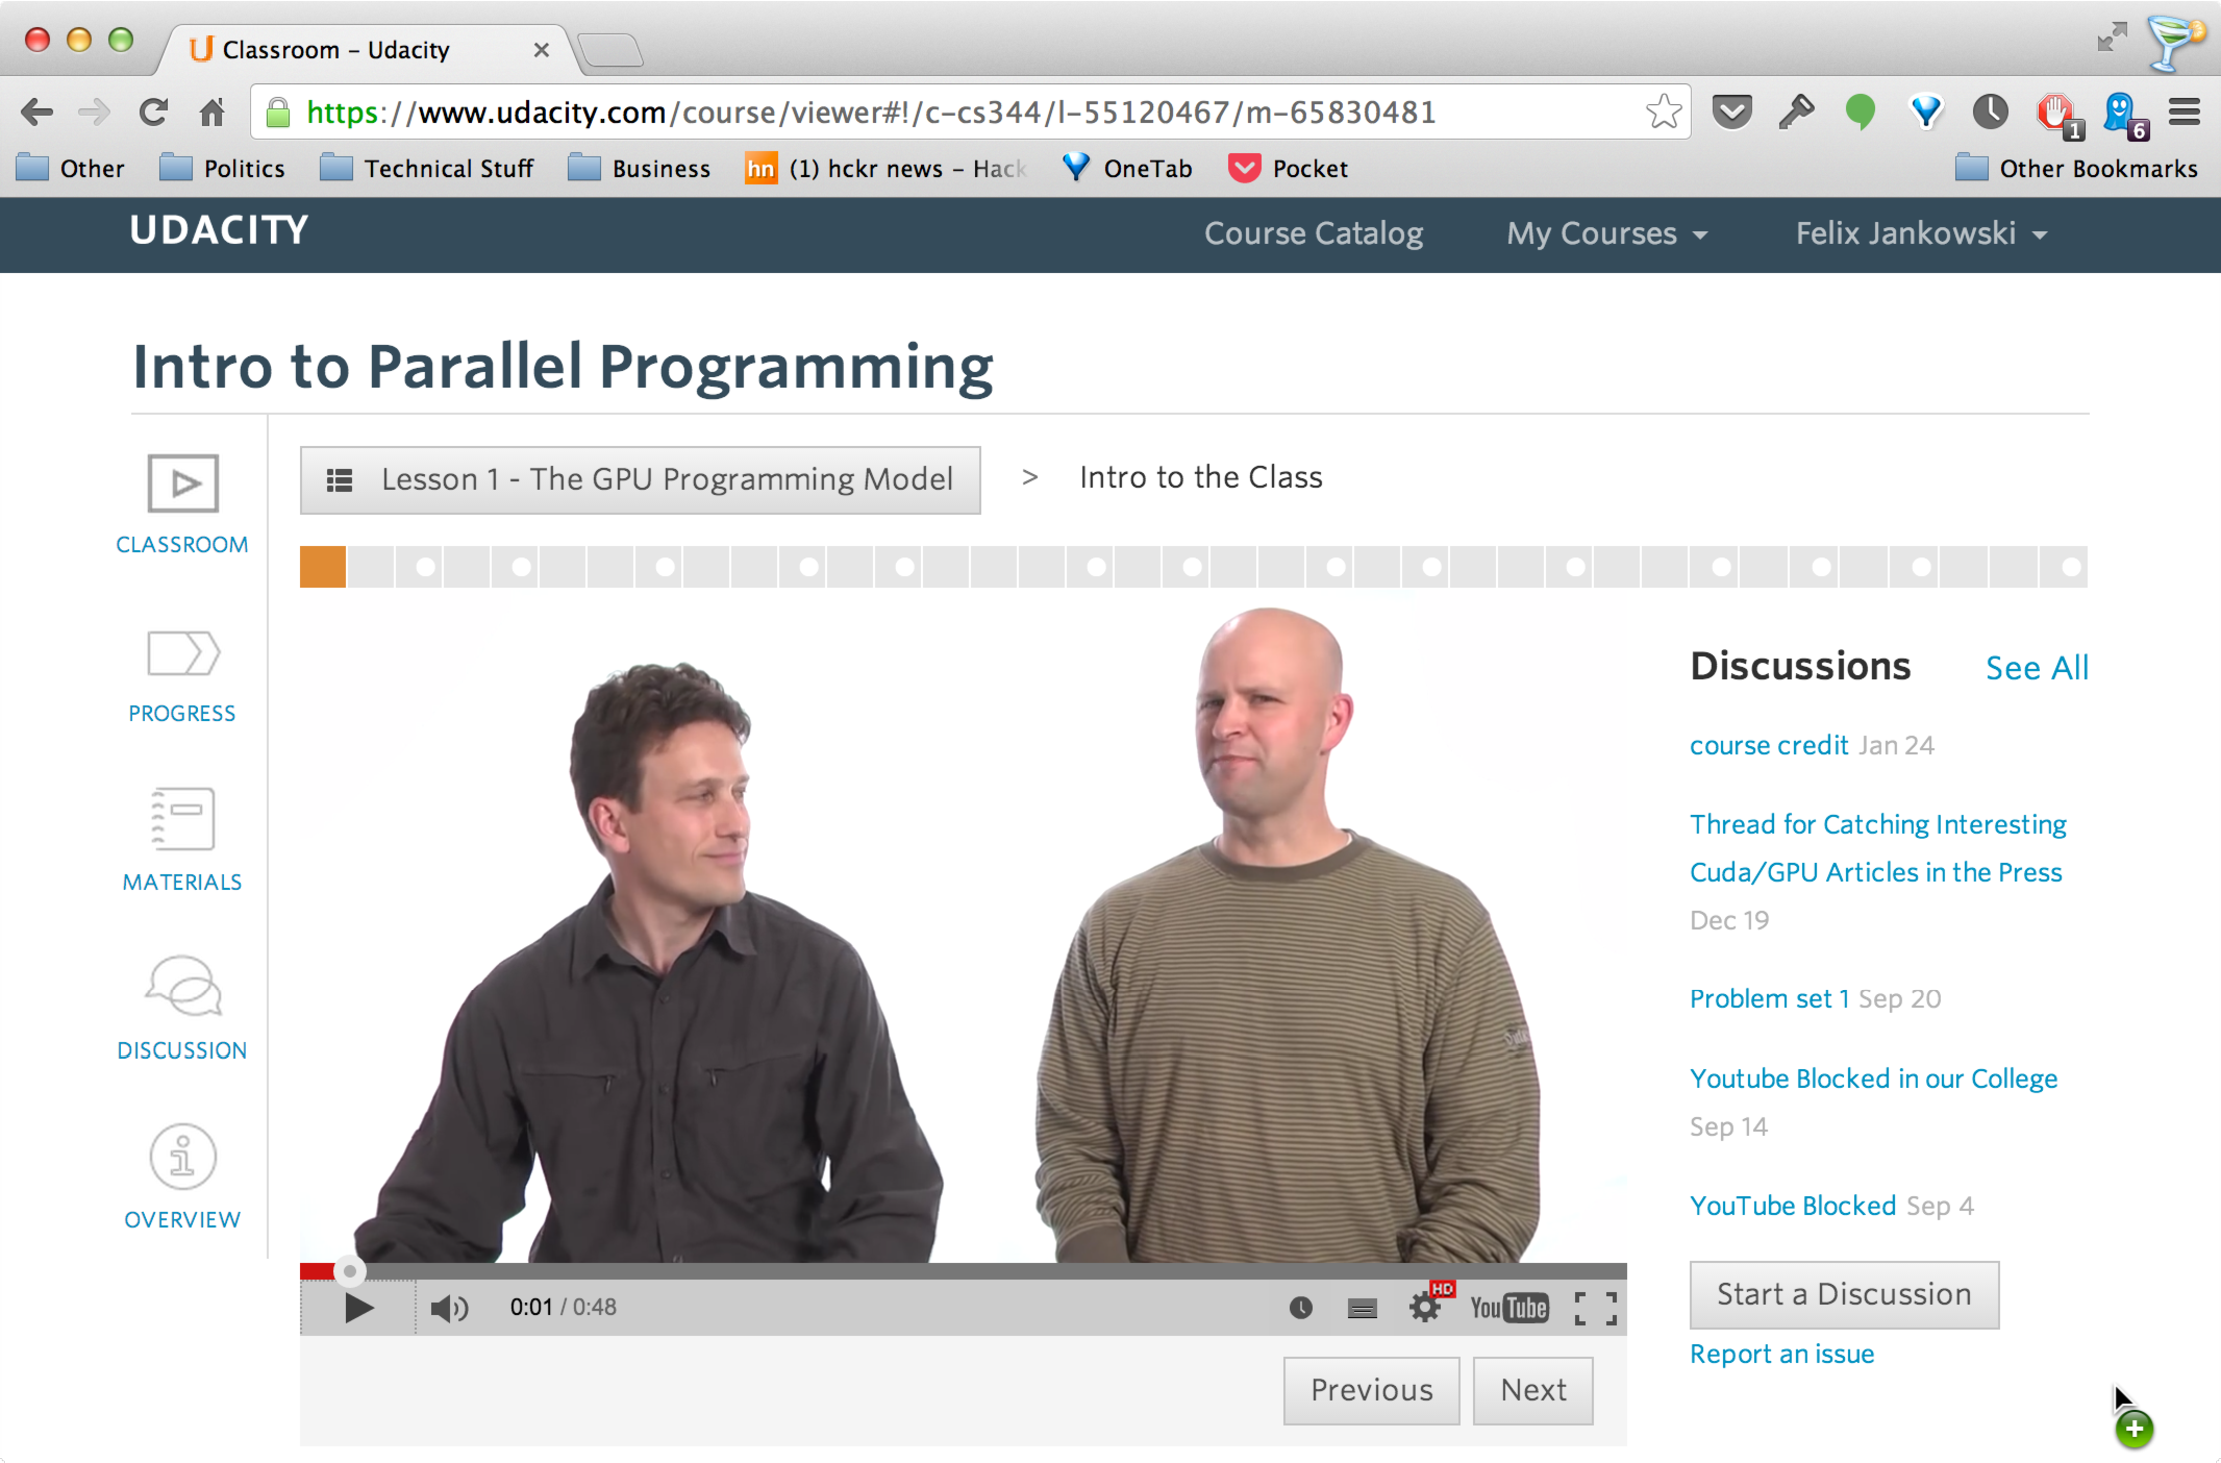
\includegraphics[width=\textwidth]{img/udacity}
					\caption{Benutzeroberfläche von Udacity}
					\label{fig:screenshot-udacity}
				\end{center}
			\end{figure}

			Besonderes Merkmal von Udacity ist, dass die Teilnehmer nach Abschluss der Lehrveranstaltungen eine Prüfung ablegen können und dafür ein Zeugnis erhalten.
			Dies wird zum Teil über Firmenkooperationen (z.B. SalesForce) angeboten, bei denen die Teilnehmer eine offizielle Zertifizierung für das jeweilige Produkt erwerben.

			Neuerdings wird in Kooperation mit der Georgia Tech University ein vollständiger Masterstudiengang in Computer Science angeboten.
			Dies ist für besonders für amerikanische Studenten attraktiv, da diese einen offiziellen akademischen Grad erwerben, ohne die zum Teil horrenden Studiengebühren in voller Höhe tragen zu müssen.

		\subsection{Coursera}

			Einen ähnlichen Ansatz verfolgt das ebenfalls von Stanford-Professoren gegründete Coursera.
			Anders als bei Udacity werden die Vorlesungen jedoch nicht von coursera selbst, sondern von zahlreichen Partneruniversitäten erstellt.
			In Deutschland nehmen die Lundwig-Maximilian-Universität München und die TU München teil\footnote{https://www.coursera.org/about/partners}. 
			Das Lehrangebot ist hierbei deutlich größer als bei Udacity, am 31. März 2014 wurden 621 Lehrveranstaltungen angeboten, wobei der größte Teil mit 114 Veranstaltungen auf den Fachbereich "`Humanities"' entfällt.


			\begin{figure}[h]
				\begin{center}
					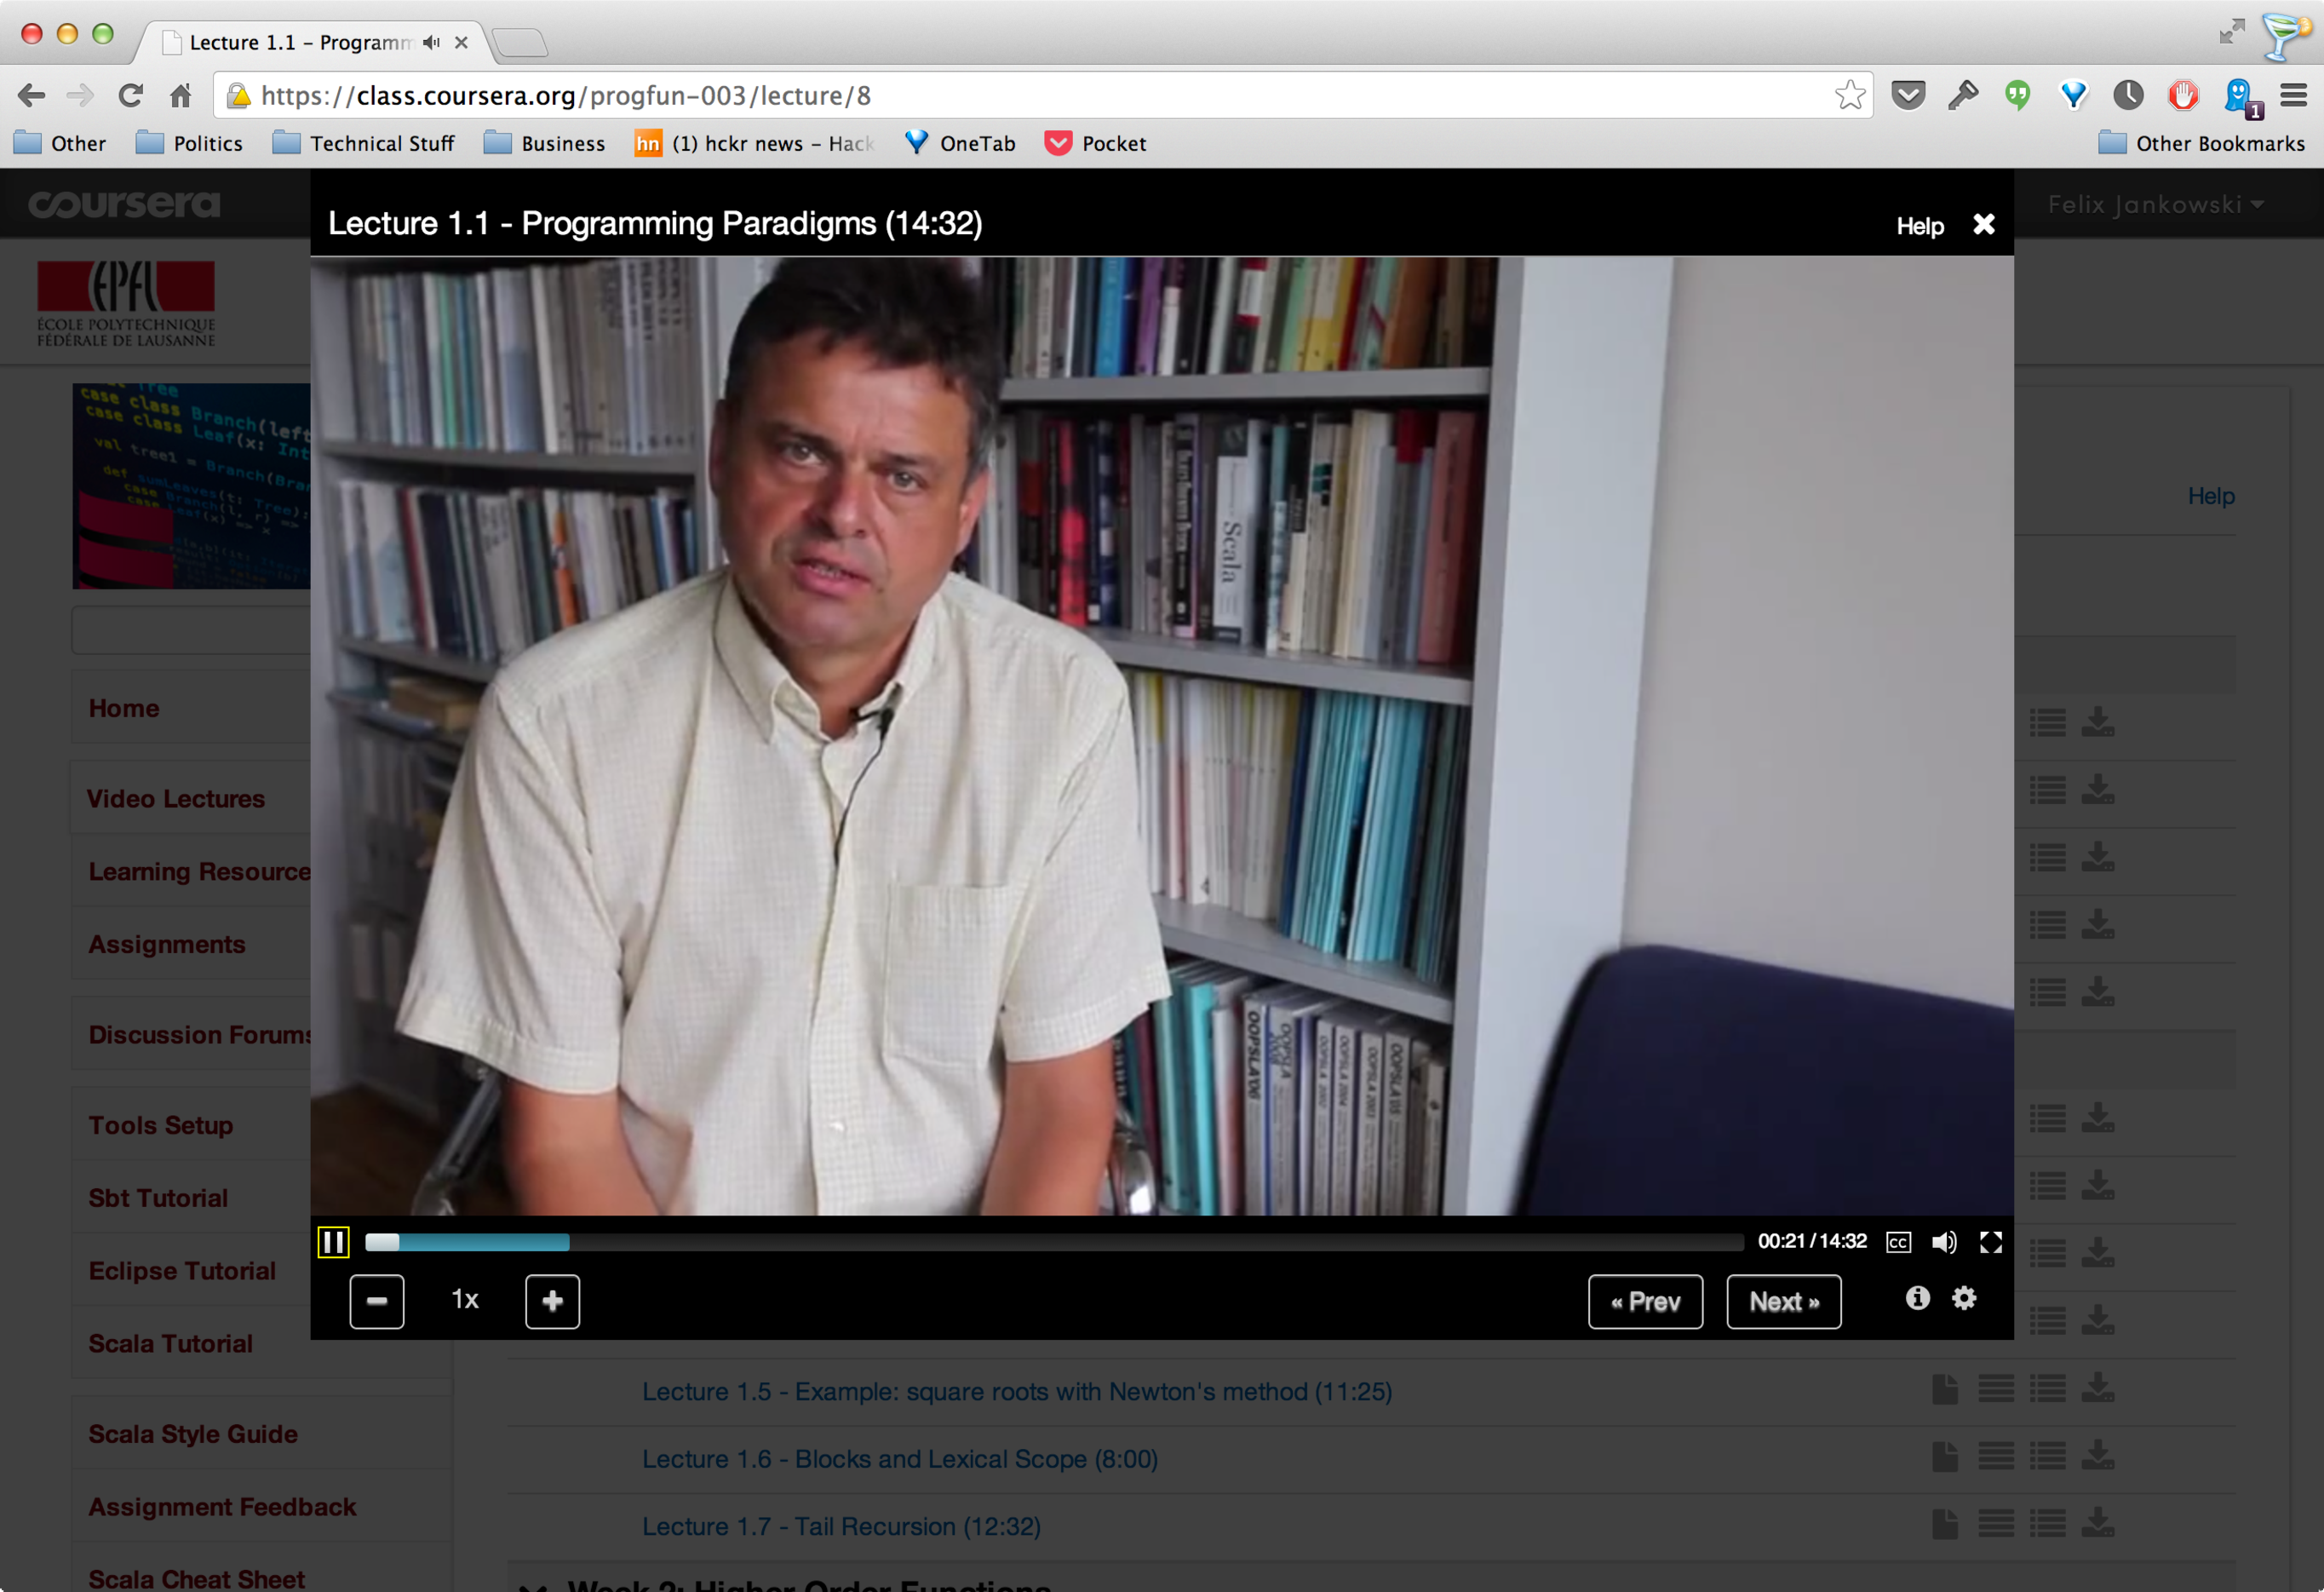
\includegraphics[width=\textwidth]{img/coursera}
					\caption{Benutzeroberfläche von Coursera}
					\label{fig:screenshot-coursera}
				\end{center}
			\end{figure}


			Die angebotene Plattform ähnelt dem Lehrbetrieb an Präsenzuniversitäten noch stärker als bei Udacity, der Hauptbestandteil sind  auf Video aufgezeichnete Vorlesungen, die von den Teilnehmern zu Hause angesehen werden sowie meist wöchentlich gestellte Übungsaufgaben, die selbstständig bearbeitet werden müssen.

			Zudem starten und enden Kurse grundsaätzlich zu festen Terminen.
			Danach werden diese archiviert, die Lehrmaterialien können nach wie vor besichtigt werden, jedoch ist keine Zertifizierung mehr möglich.
			Dies ist für berufstätigen Personen von Nachteil, da diese nicht immer ausreichend Möglichkeiten zur Einhaltung der Fristen zur Verfügung haben und keine Rücksicht auf das individuelle Lerntempo und die freie Zeit genommen werden kann.
			Ein weiterer Kritikpunkt bei coursera ist, dass die Bewertung von Übungsaufgaben durch andere Teilnehmer erfolgt.
			Diese sind gelegentlich unzutreffend und frustrieren somit die Teilnehmer.
			Entsprechend gering ist die Erfolgsquote, nach Medienberichten werden Lehrveranstaltungen von über 90\% der Teilnehmer vorzeitig abgebrochen. 


%%%%%%%%%%%%%%%%%%%%%%%%%%%%%%%%%%%%%%%%%%%%%%%%%%%%%%%%%%%%%%%%%%%%%%%%%%%%%%%%%%%%%%%%%%%%%%%%%%%%%%%%%
\section{Technologien}
\label{sec:technologies}
%%%%%%%%%%%%%%%%%%%%%%%%%%%%%%%%%%%%%%%%%%%%%%%%%%%%%%%%%%%%%%%%%%%%%%%%%%%%%%%%%%%%%%%%%%%%%%%%%%%%%%%%%


		Betrachtet wird ausschließlich die Intel x86-Plattform.
		Diese Plattform wurde von Microsoft durchgängig unterstützt, seit MS DOS für den ersten IBM PC, der mit einem Intel 8088 ausgestattet war, ausgeliefert wurde.
		Durch den enormen Erfolg dieses PCs und seiner Klone wurde diese Architektur schnell zur am weitesten Verbreiteten und kommerziell Erfolgreichsten.
		Die Weiterentwicklung, meist unter Federführung durch Intel, erfolgte stetig und konsequent. 
		Trotzdem wird bis heute auf Binärkompatibilität geachtet, wodurch der Betrieb von historischer Software ohne Emulation der CPU ermöglicht wird. 
		
		Die Virtualisierung eines Computers dieser Plattform in Software gestaltet sich jedoch nicht unkompliziert.
		Das durch \cite{PopekGoldberg} aufgestellte erste Virtualisierungstheorem besagt in vereinfachter Form, dass eine effiziente Virtualisierung möglich ist, sofern alle privilegierten Instruktionen einen Exception auslösen, falls diese im User Mode ausgeführt werden.
		Somit kann die Anweisung abgefangen und durch den Hypervisor emuliert werden. 
		Dies ist bei x86 jedoch nicht der Fall.
		So existieren laut \cite{PentiumVirt} in der IA-32, der beim Pentium verwendeten Weiterentwicklung von x86, insgesamt 17 Operationen, die diese Bedingung verletzen.
		Diese schlagen entweder fehl ohne eine Exception auszulösen oder zeigen unterschiedliches Verhalten im User bzw. im Kernel Mode.

		Derartige Spezialfälle müssen vom Hypervisor durch binäres Umschreiben (binary translation / binary rewriting) abgefangen werden. 
		Dabei wird der Programmcode der ausgeführten Software in Echtzeit so verändert, dass diese Anweisungen umgangen und das Verhalten einer nativen CPU emuliert werden kann. 
		Interessant hierbei ist, dass einige Operationen effizienter in Software als in Hardware ausführbar sind und damit die virtualisierten Hosts in manchen Fällen bessere Performanceeigenschaften zeigen als beim Betrieb direkt auf Hardware.

		Im Jahr 2005 wurden die Befehlssatzerweiterungen AMD-V and Intel VT-x eingeführt.
		Mit diesen ist es möglich x86-kompatible CPUs in einem Modus zu betreiben, in dem die Popek und Goldberg Virtualisierungstheoreme erfüllt werden. 
		Durch diese Hardwareunterstützung kann auf das fehlerbehaftete binäre Umschreiben gänzlich verzichtet werden.

		% Typ 1/2 Virtualisierung (hier ggf. nicht relevant)


		%%%%%%%%%%%%%%%%%%%%%%%%%%%%%%%%%%%%%%%%%%%%%%%%%%%%%%%%%%%%
		\subsection{VMWare}
		%%%%%%%%%%%%%%%%%%%%%%%%%%%%%%%%%%%%%%%%%%%%%%%%%%%%%%%%%%%%

		Das Unternehmen VMWare wurde im Jahr 1998 gegründet mit dem Ziel, die Virtualisierung von x86-basierten Computern zu ermöglichten.
		Im Juli 1999 veröffentlichte es VMWare Workstation, den erste für Endanwernder funktionsfähige Hypervisor unter Microsoft Windows auf x86.

		Mit diesem auch kommerziell sehr erfolgreichen Produkt wurde Virtualisierung außerhalb von Mainframes möglich und bekannt. 
		Insbesondere die Betriebssystem- und Treiberentwicklung konnte stark vereinfacht werden. 

		Aufgrund der langen Erfahrung dieses Unternehmens werden die Produkte von vielen Personen nach wie vor als qualitativ führend angesehen. 
		Besonders die clientseitigen Treiber erreichen beste Performance und Stabilitätswerte.
		Auch gilt das VMWare Format, in dem die Images gespeichert werden, als eine Art de-facto-Standard und kann von fast allen anderen Produkten importiert werden.

		Zudem werden durch den frühen Entwicklungsbeginn historische Betriebssysteme am besten unterstützt.
		Beispielsweise wurde Windows NT 4 im Jahr 2000 durchaus noch häufig kommerziell eingesetzt.

		Aus diesen Gründen wird im Rahmen dieser Arbeit zunächst versucht, die Ziele mit Hypervisoren von VMWare zu erreichen.

		%%%%%%%%%%%%%%%%%%%%%%%%%%%%%%%%%%%%%%%%%%%%%%%%%%%%%%%%%%%%
		\subsection{KVM}
		%%%%%%%%%%%%%%%%%%%%%%%%%%%%%%%%%%%%%%%%%%%%%%%%%%%%%%%%%%%%


		Einen anderen Ansatz geht die Kernel-based Virtual Machine (KVM) von Linux, welche dieses zu einem Hypervisor erweitert. 
		Anders als VMWare und die meisten anderen Produkte unterstützt diese kein binäres Umschreiben und benötigt somit Hardwareunterstützung.

		Auch bietet sie kein User Interface sondern erzeugt mit $/dev/kvm$ lediglich ein virtuelles Device, über das eine Anwendung im User Mode auf den Hypervisor zugreifen kann.
		Diese kann somit neue virtuelle Maschinen anlegen und konfigurieren, mit diesen kommunizieren und ihren Video-Output anzeigen, ohne selbst Operationen im Kernel Mode durchführen zu müssen.

		Mittlerweile gibt es zahlreiche Clientanwendungen, die meist für Zugriff aus der Ferne optimiert sind. 
		Workstation-ähnliche Funktionalität kann jedoch mit dem Emulator QEMU erreicht werden.
		Besonders gut funktioniert KVM mit Linux als Gastbetriebssystem, da der Kernel bereits zahlreiche hochwertige Treiber zur Paravirtualisierung mitbringt, die meist von den gleichen Entwicklern wie KVM selbt gewartet werden.
		Mit dem VirtIO Framework ist auch Paravirtualisierung von Windows-Guests möglich, welches aber nicht an die VMWare Guest Additions heranreicht.
		%Insbesondere fehlt eine Hardwarebeschleunigung für 3D Grafik, weswegen zahlreiche Programme schlecht und nur sehr langsam gerendert werden können.

		Aufgrund der großen Verbreitung von Linux im Serverbereich und unter Profis erfreut sich KVM zunehmender Beliebtheit.
		Hauptanwendungszweck ist wegen der o.g. Einschränkungen die Bereitstellung von Linux-Guests in einem Cloud-Computing Umfeld.
		Meist kommt dabei libVirt, eine universelle Bibliothek zur Konfiguration und zum Betrieb verschiedener Hypervisoren zum Einsatz. 
		
		Wegen der freien und quelloffenen Verfügbarkeit verwendet die zur Zeit in Betrieb befindliche Version von InstantLab ebenfalls KVM auf ihren execution hosts. 
		Daher wird es in dieser Arbeit ebenfalls berücksichtigt.
